\section{Метод №1}\label{meth1}

\subsection{Идея}\label{math1:idea}

\begin{itemize}
	\item[1)] Аппроксимируем множества точек прямыми.
	\item[2)] Проводим плоскости через полученные прямые и направления проектирования и получаем некую призму в пересечении трех плоскостей.
	\item[3)] Ищем прямую, минимально удаленную от данных трех плоскостей. 
\end{itemize}

\begin{center}
	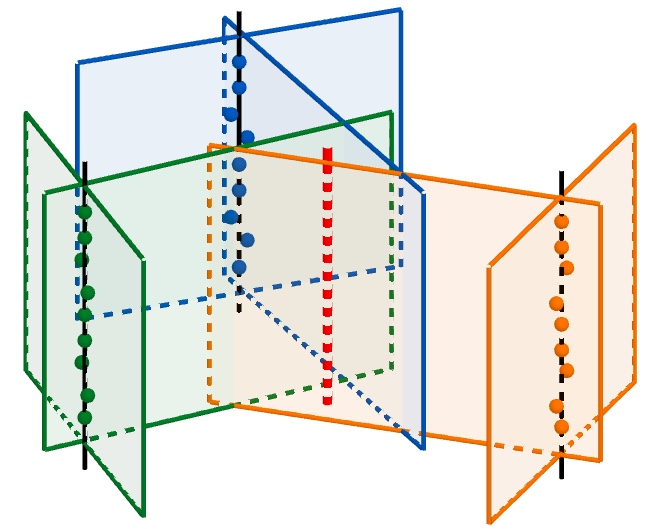
\includegraphics[scale=0.7]{11}

	Рис. 2.1: Построение прямых и плоскостей через точки множеств.
\end{center}

\subsection{Решение}\label{math1:solution}

Пусть имеем три множества:

\begin{center}
	$P_1 = \Set{p_i^1 = (x_i^1, y_i^1, z_i^1)}{i=\ton n_1}$

	\vspace{0.3cm}
	$P_2 = \Set{p_i^2 = (x_i^2, y_i^2, z_i^2)}{i=\ton n_2}$

	\vspace{0.3cm}
	$P_3 = \Set{p_i^3 = (x_i^3, y_i^3, z_i^3)}{i=\ton n_3}$
\end{center}

Используя алгоритм аппроксимации множества точек прямой \ref{line:alg:3dim}, получаем три прямые, приближающие наши множества $P_1$, $P_2$ и $P_3$:

\begin{center}
	$\mathit{l_1}: \; \begin{cases}
		x = x_0^1 + m^1 \cdot t \\
		y = y_0^1 + n^1 \cdot t \\
		z = z_0^1 + p^1 \cdot t
	\end{cases}$, где $t \in \mathbb{R}$ - параметр. 
\end{center}

\begin{center}
	$\mathit{l_2}: \; \begin{cases}
		x = x_0^2 + m^2 \cdot t \\
		y = y_0^2 + n^2 \cdot t \\
		z = z_0^2 + p^2 \cdot t
	\end{cases}$, где $t \in \mathbb{R}$ - параметр. 
\end{center}

\begin{center}
	$\mathit{l_3}: \; \begin{cases}
		x = x_0^3 + m^3 \cdot t \\
		y = y_0^3 + n^3 \cdot t \\
		z = z_0^3 + p^3 \cdot t
	\end{cases}$, где $t \in \mathbb{R}$ - параметр. 
\end{center}

Пусть $(m_1, n_1, p_1)^T$, $(m_2, n_2, p_2)^T$, $(m_3, n_3, p_3)^T$ - направления проектирования.

Тогда плоскости через найденные прямые и направления проектирования имеют вид:

\begin{center}
	$\mathit{\pi_1}: \; \begin{cases}
		x = x_0^1 + m^1 \cdot t_1 + m_1 \cdot t_2 \\
		y = y_0^1 + n^1 \cdot t_1 + n_1 \cdot t_2 \\
		z = z_0^1 + p^1 \cdot t_1 + p_1 \cdot t_2
	\end{cases}$, где $t_1, t_2 \in \mathbb{R}$ - параметры. 
\end{center}

\begin{center}
	$\mathit{\pi_2}: \; \begin{cases}
		x = x_0^2 + m^2 \cdot t_1 + m_2 \cdot t_2 \\
		y = y_0^2 + n^2 \cdot t_1 + n_2 \cdot t_2 \\
		z = z_0^2 + p^2 \cdot t_1 + p_2 \cdot t_2
	\end{cases}$, где $t_1, t_2 \in \mathbb{R}$ - параметры. 
\end{center}

\begin{center}
	$\mathit{\pi_3}: \; \begin{cases}
		x = x_0^3 + m^3 \cdot t_1 + m_3 \cdot t_2 \\
		y = y_0^3 + n^3 \cdot t_1 + n_3 \cdot t_2 \\
		z = z_0^3 + p^3 \cdot t_1 + p_3 \cdot t_2
	\end{cases}$, где $t_1, t_2 \in \mathbb{R}$ - параметры. 
\end{center}

Используя алгоритм нахождения прямой, минимально удаленной от данного множества плоскостей \ref{plane:alg:3dim}, получаем искомый отрезок (прямую).

\subsection{Погрешность и примеры работы программ}\label{math1:error}

Погрешность метода состоит из погрешности аппроксимации множеств точек прямыми и погрешности нахождения прямой, минимально удаленной от данного множества прямых.

\subsubsection{Искусственные данные}\label{math2:error:synth}

Исходные данные - три множетсва точек и три направления проектирования:

\begin{verbatim}
	(2, -4, 0)	          (-4, 2, 0)            (6.242641, 6.242641, 0)
	(2.1, -4, 1)         (-4, 2.1, 1)          (6.342641, 6.142641, 1)
	(1.9, -4, 2)         (-4, 1.9, 2)          (6.242641, 6.242641, 1.5)
	(2, -4, 3)           (-4, 2, 3)            (6.142641, 6.342641, 2)
	(2, -4, 4)           (-4, 2, 4)            (6.242641, 6.242641, 3)
	(2.1, -4, 5)         (-4, 2.1, 5)          (6.242641, 6.242641, 4)
	(1.9, -4, 6)         (-4, 1.9, 6)          (6.342641, 6.142641, 5)
	(2, -4, 7)           (-4, 2, 6.5)          (6.142641, 6.342641, 6)
	(2, -4, 7.5)         (-4, 2, 7)            (6.242641, 6.242641, 7)
	(2, -4, 8)           (-4, 2, 8)            (6.242641, 6.242641, 8)

	(0, 1, 0)            (1, 0, 0)             (-0.707107, -0.707107, 0)
\end{verbatim}

Полученные данные - направляющие векторы и точки прямых, аппроксимирующих исходные множества, а также две точки искомой прямой и значение функционала:

\begin{multicols}{2}
	\begin{verbatim}
		vector of line 1:
		(-0.002817, -0.000000, 1.000000)
		vector of line 2:
		(-0.000000, -0.003049, 1.000000)
		vector of line 3:
		(-0.003051, 0.003051, 1.000000)
	\end{verbatim}
	\columnbreak

	\begin{verbatim}
		point of line 1:
		(2.000001, -4.000001, 4.350000)
		point of line 2:
		(-4.000001, 2.000001, 4.250000)
		point of line 3:
		(6.242641, 6.242641, 3.750000)
\end{verbatim}
\end{multicols}
\begin{verbatim}
	TWO POINTS OF RESULT LINE:
	2.012064 2.000192 0.000000
	1.989034 2.000686 8.000000
	Lambda = 0.005286
\end{verbatim}

\begin{center}
	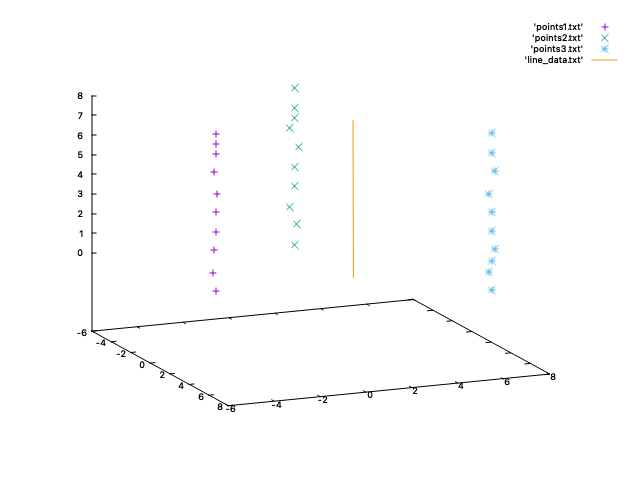
\includegraphics[scale=0.7]{meth1synth}
	\textit{полученный отрезок и исходные множества}
\end{center}

\begin{center}
	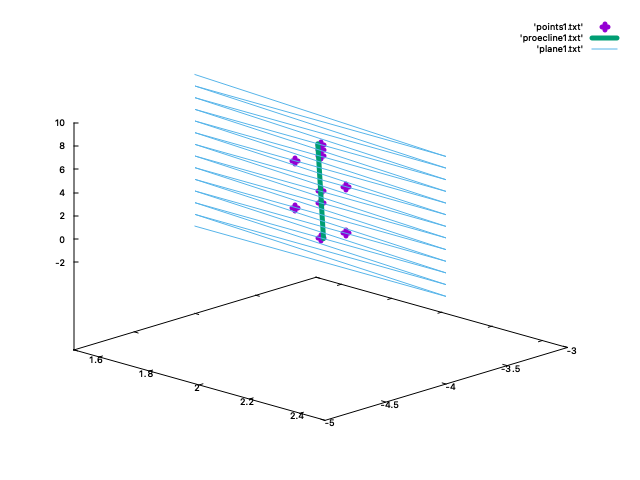
\includegraphics[scale=0.65]{meth1synthproec1}

	\textit{проекция полученного отрезка на плоскость первого множества}
	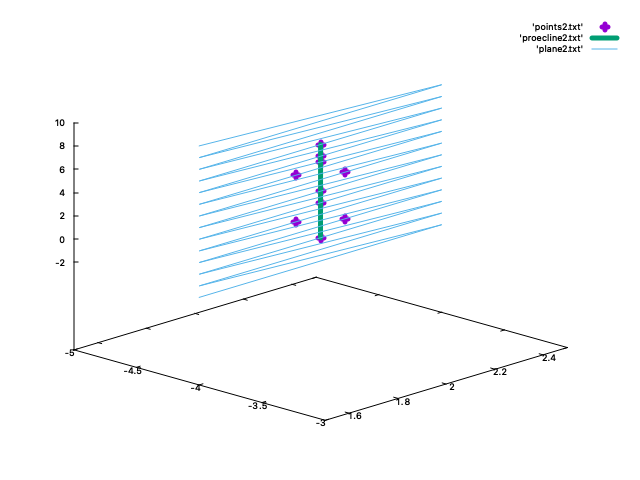
\includegraphics[scale=0.65]{meth1synthproec2}

	\textit{проекция полученного отрезка на плоскость второго множества}
	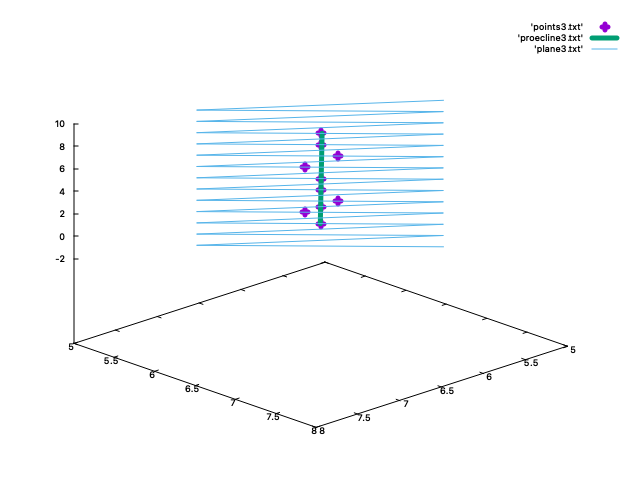
\includegraphics[scale=0.65]{meth1synthproec3}
	
	\textit{проекция полученного отрезка на плоскость третьего множества}
\end{center}

\subsubsection{Реальные данные}\label{math2:error:real}

Исходные данные - 100 множетсв точек и 100 направлений проектирования отрезка, ограниченного по $z$ значениями $-6.08332812434530$ и $-4.57712089734895$. Фигура симметричная, поэтому имеем два искомых отрезка.\\

Полученные данные - по две точки искомых прямых и значения функционала:

\begin{verbatim}
			DATA FOR POSITIVE SET:
	(3.227280, 2.584213, -6.083328)
	(2.505698, 1.505435, -4.577121)
	Lambda = 0.000003
			DATA FOR NEGATIVE SET:
	(-2.979147, -2.780110, -6.083328)
	(-2.377633, -1.727098, -4.577121)
	Lambda = 0.000030
\end{verbatim}

\begin{center}
	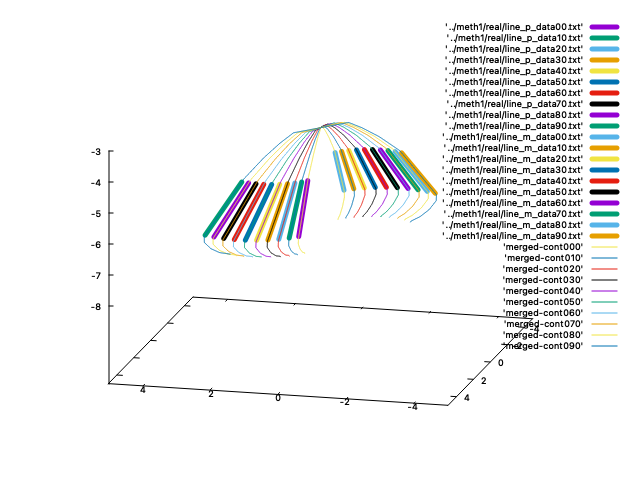
\includegraphics[scale=0.8]{meth1lineapprox}

	\textit{прямые, аппорксимирующие множества точек}

	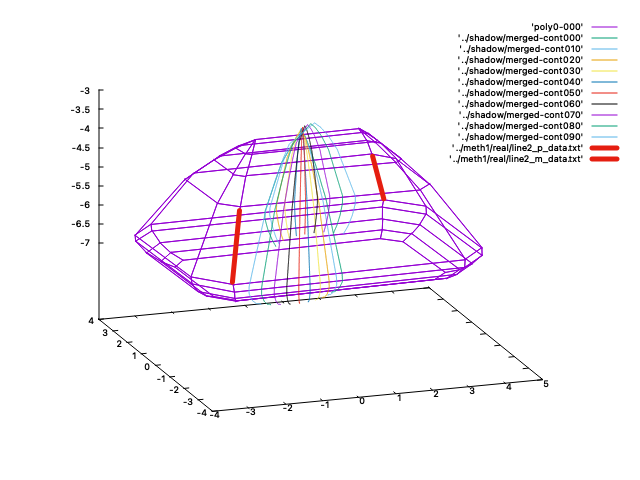
\includegraphics[scale=0.7]{meth1realresult}

	\textit{искомые отрезки, идеальный контур фигуры и исходные контуры проекций}

	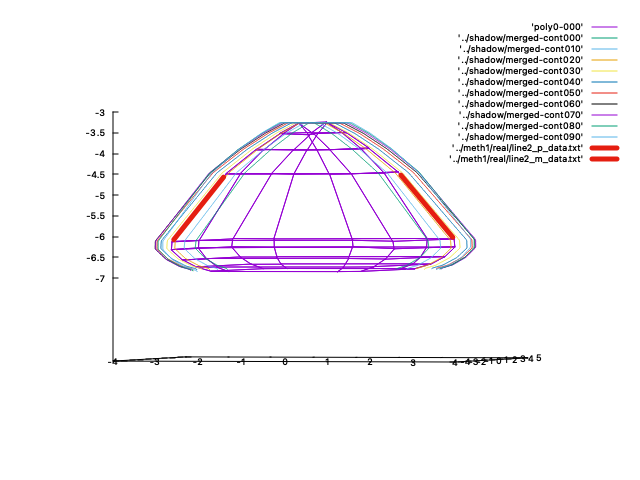
\includegraphics[scale=0.7]{meth1realsideview}

	\textit{искомые отрезки, идеальный контур фигуры и исходные контуры проекций}
\end{center}

\newpage